\documentclass{homework}
\usepackage{homework}
\usepackage{pdfpages}

\title{COC473 - Lista 6}
\author{Pedro Maciel Xavier}
\register{116023847}
\notes{\textbf{Nota:} Na primeira seção da Lista estão os trechos de código dos programas pedidos. Na segunda parte, estão os resultados dos programas assim como a análise destes. Por fim, no apêndice está o código completo. Caso os gráficos estejam pequenos, você pode ampliar sem problemas pois foram renderizados diretamente no formato \texttt{.pdf}.}

\newcommand{\vecx}[3]{
	\ensuremath{\left[\begin{array}{@{}c@{}}
			#1\\
			#2\\
			#2
		\end{array}\right]}
}

\begin{document}
	
	\maketitle
	
	\section*{Programas}
	
	\questx[{Escreva um programa que "integre" uma equação diferencial ordinária de primeira ordem $y'(t) = f(t, y(t))$ onde o usuário pode escolher o método de solução entre as três seguintes possibilidades:%%
	\begin{enumerate}[label=\alph*)]%%
		\item \textit{Euler}
		\item \textit{Runge-Kutta} de segunda ordem
		\item \textit{Runge-Kutta} de quarta ordem
	\end{enumerate}~
	}]%%1
	
	A função \code{ode\_solve(df, y0, t, n, kind)} integra a função \code{df} sobre o domínio do tempo definido pelo vetor \code{t[n]}, assumindo que o valor de $y(t)$ correspondente a primeira entrada de \code{t[n]} é \code{y0}. O argumento nomeado opcional \code{kind} define o método a ser utilizado:
	\begin{itemize}[leftmargin=100pt]
		\item[\code{'euler'}] \textit{Euler}
		\item[\code{'runge-kutta2'}] \textit{Runge-Kutta} de segunda ordem
		\item[\code{'runge-kutta4'}] \textit{Runge-Kutta} de quarta ordem
	\end{itemize}
	
	\lstinputlisting[firstline=882, lastline=988, style=fortranstyle, gobble=0]{../src/calclib.f95}
	
	\newpage
	
	\section*{Aplicações}
	
	\questx[Utilizando o programa desenvolvido, use os métodos de \textit{Euler}, \textit{Runge-Kutta} de segunda ordem e \textit{Runge-Kutta} de quarta ordem, para $0 \le t \le 10$, e resolva a seguinte equação diferencial ordinária:%%
	\begin{align*}%%
		y'(t) &= -2 t y(t)^2\\
		y(0) &= 1
	\end{align*}%%
	Compare com a solução exata $\displaystyle y(t) = \frac{1}{1 + t^2}$]
	
	\begin{fig}
		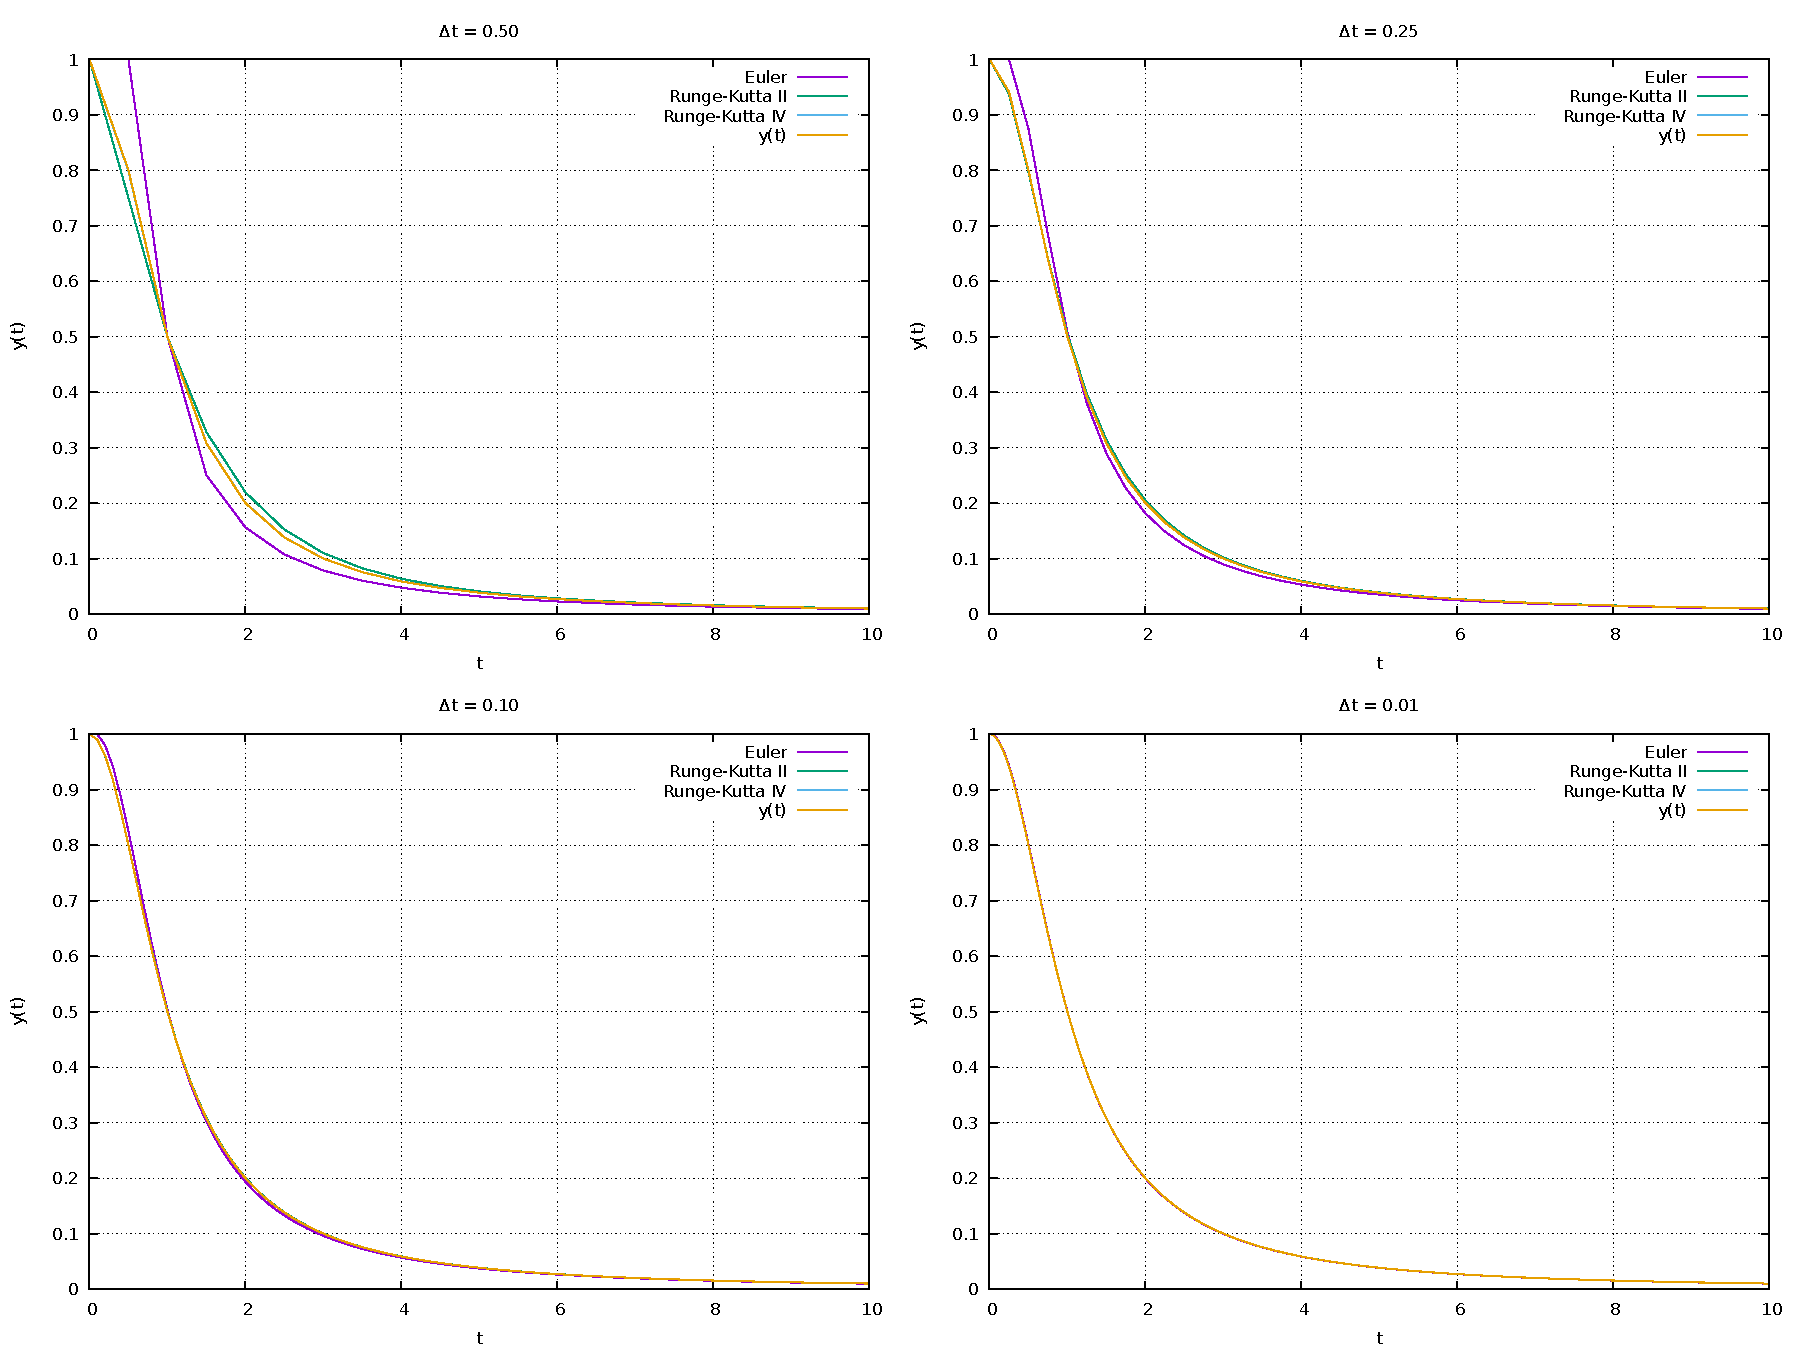
\includegraphics[width=\textwidth]{../src/plot/L6-Q1.pdf}
	\end{fig}
	
	Vemos neste caso que o método de \textit{Runge-Kutta} de quarta ordem converge muito rapidamente para a solução ao longo de toda a curva, sendo difícil distinguir seu gráfico daquele que descreve a solução. O método de segunda ordem é o próximo a garantir sua convergência. Por fim, o método de \textit{Euler} se aproxima da solução para passos ainda menores, uma ordem de grandeza abaixo dos demais.\par
	
	É interessante notar, neste caso, que apesar de se distanciarem da solução no meio do percurso, as aproximações numéricas atingem valores muito próximos ao fim do processo, mesmo com passos mais generosos.
	
	\newpage
	
	\section*{Programas}
	
	\questx[{Escreva um programa que "integre" uma equação diferencial ordinária de segunda ordem $y''(t) = f(t, y(t), y'(t))$ onde o usuário pode escolher o método de solução entre as seguintes possibilidades:%%
		\begin{enumerate}[label=\alph*)]%%
			\item Aproximação de segunda ordem em Série de \textit{Taylor}
			\item \textit{Runge-Kutta-Nystrom}
		\end{enumerate}~
	}]%%1]

	A função \code{ode2\_solve(d2f, y0, dy0, t, n, kind)} integra a função \code{d2f} sobre o domínio do tempo definido pelo vetor \code{t[n]}, assumindo que o valor de $y(t)$ correspondente a primeira entrada de \code{t[n]} é \code{y0} e que o valor de $y'(t)$ neste mesmo ponto é \code{dy0}. O argumento nomeado opcional \code{kind} define o método a ser utilizado:
	\begin{itemize}[leftmargin=100pt]
		\item[\code{'taylor'}] Aproximação em Série de \textit{Taylor}
		\item[\code{'runge-kutta-nystrom'}] Método de \textit{Runge-Kutta-Nystrom}
	\end{itemize}
	
	\lstinputlisting[firstline=990, lastline=1077, style=fortranstyle, gobble=0]{../src/calclib.f95}
	
	\newpage
	
	\section*{Aplicações}
	
	\questx[{Resolva a seguinte equação diferencial pelos métodos 'Expansão em Série de \textit{Taylor}' e \textit{Runge-Kutta-Nystrom}, $0 \le t \le 100$, utilizando o programa desenvolvido na Tarefa 02:%
	\begin{align*}%%
		&m y''(t) + c y'(t) + k y(t) = F(t)\\
		&m = 1; c = 0.2; k = 1;\\
		&F(t) = 2 \sin (w t) + \sin (2 w t) + cos (3 w t)\\
		&w = 0.5;\\
		&y'(0) = y(0) = 0.0
	\end{align*}%%
	}]

	\begin{fig}
		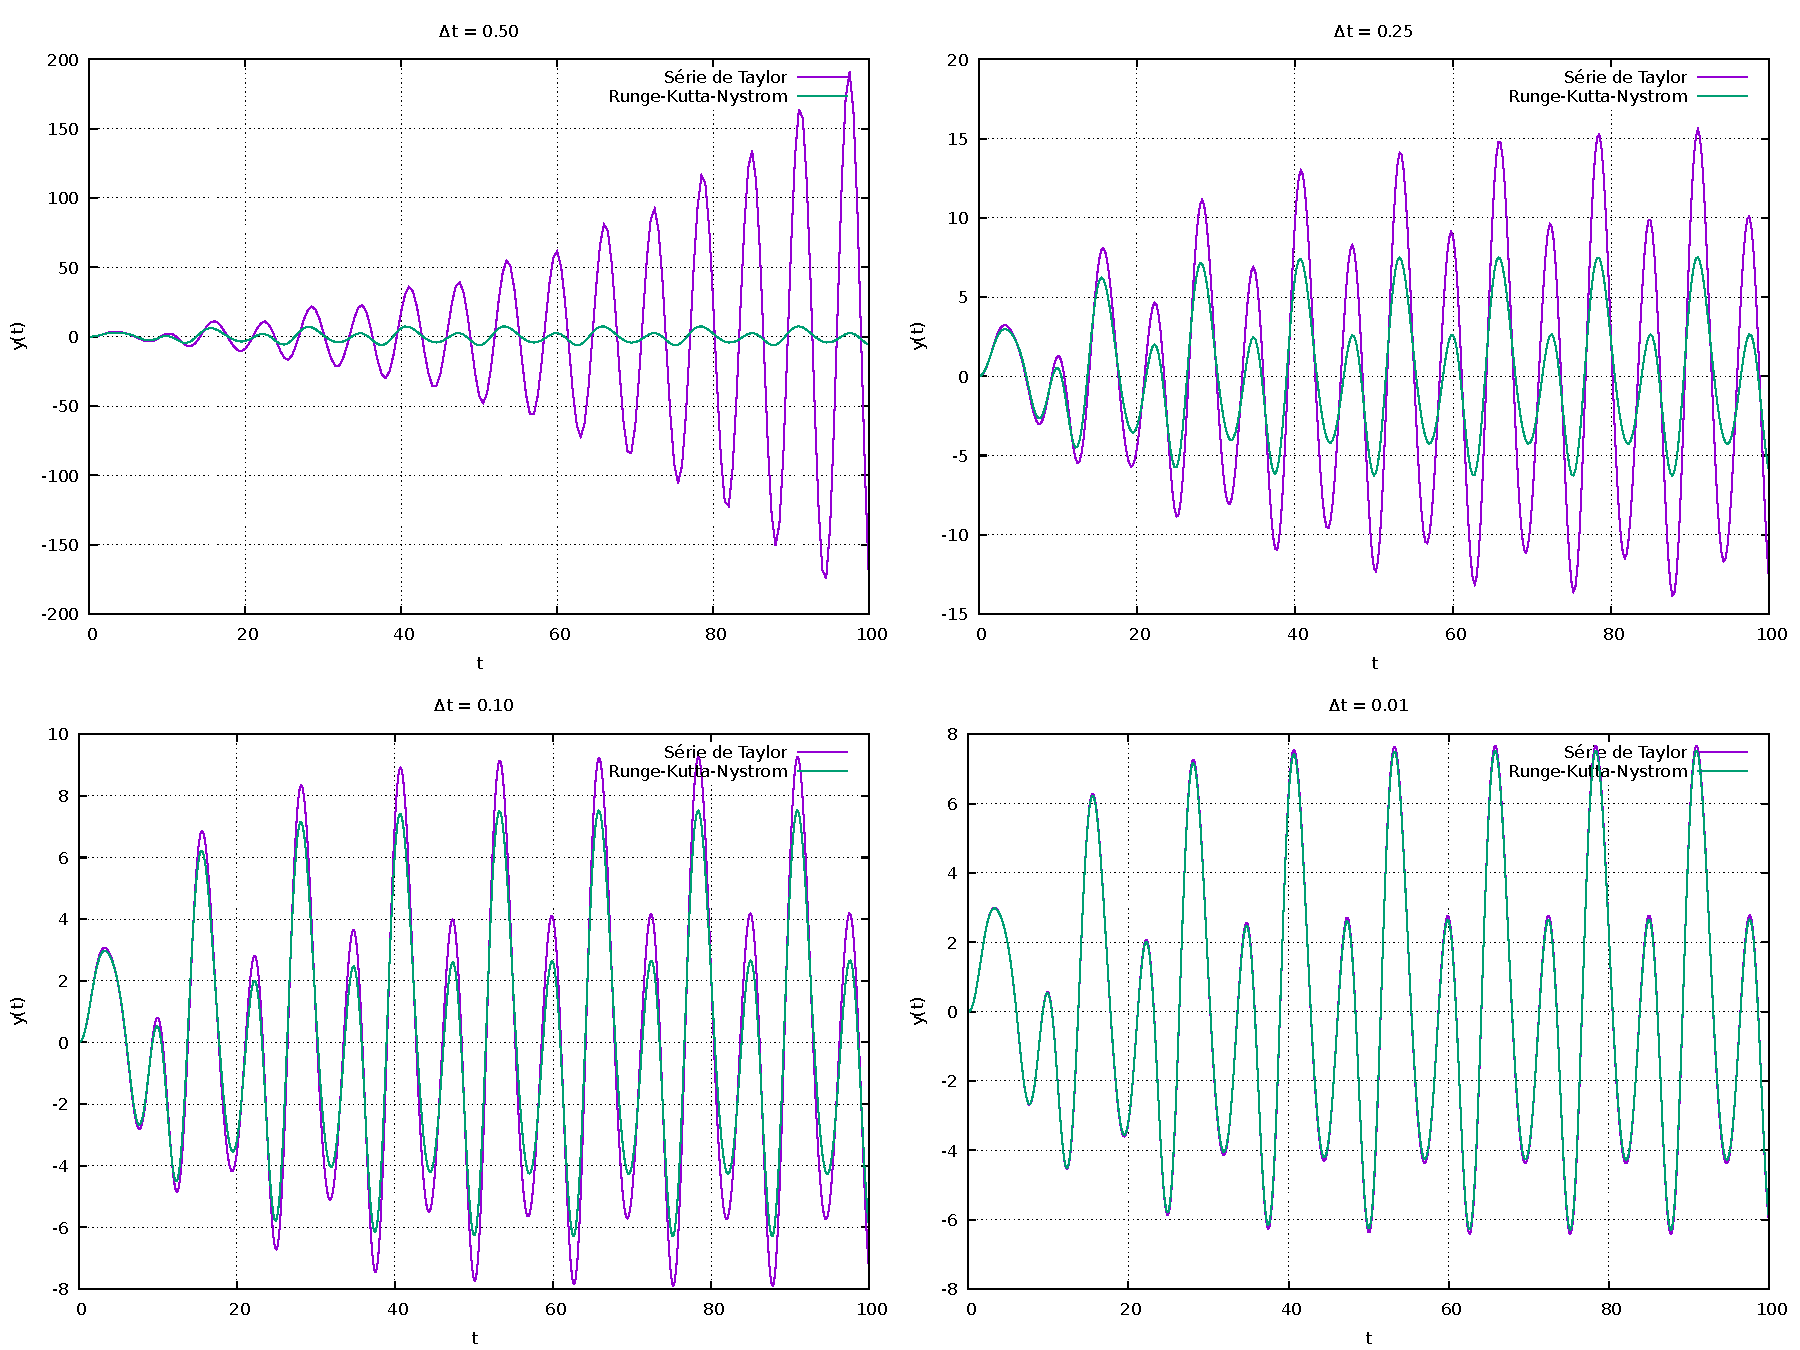
\includegraphics[width=\textwidth]{../src/plot/L6-Q2.pdf}
	\end{fig}

	\quest[{Resolva a equação diferencial de segunda ordem apresentada em sala de aula pelos métodos 'Expansão em Série de \textit{Taylor}' e \textit{Runge-Kutta-Nystrom}, $0 \le t \le 20$, utilizando o programa desenvolvido na Tarefa 02:%
	\begin{align*}%%
		&z''(t) = - g - k \cdot z'(t) \cdot |z'(t)|\\
		&k = 1;\\
		&z'(0) = z(0) = 0
	\end{align*}%%
	}]

	\begin{fig}
		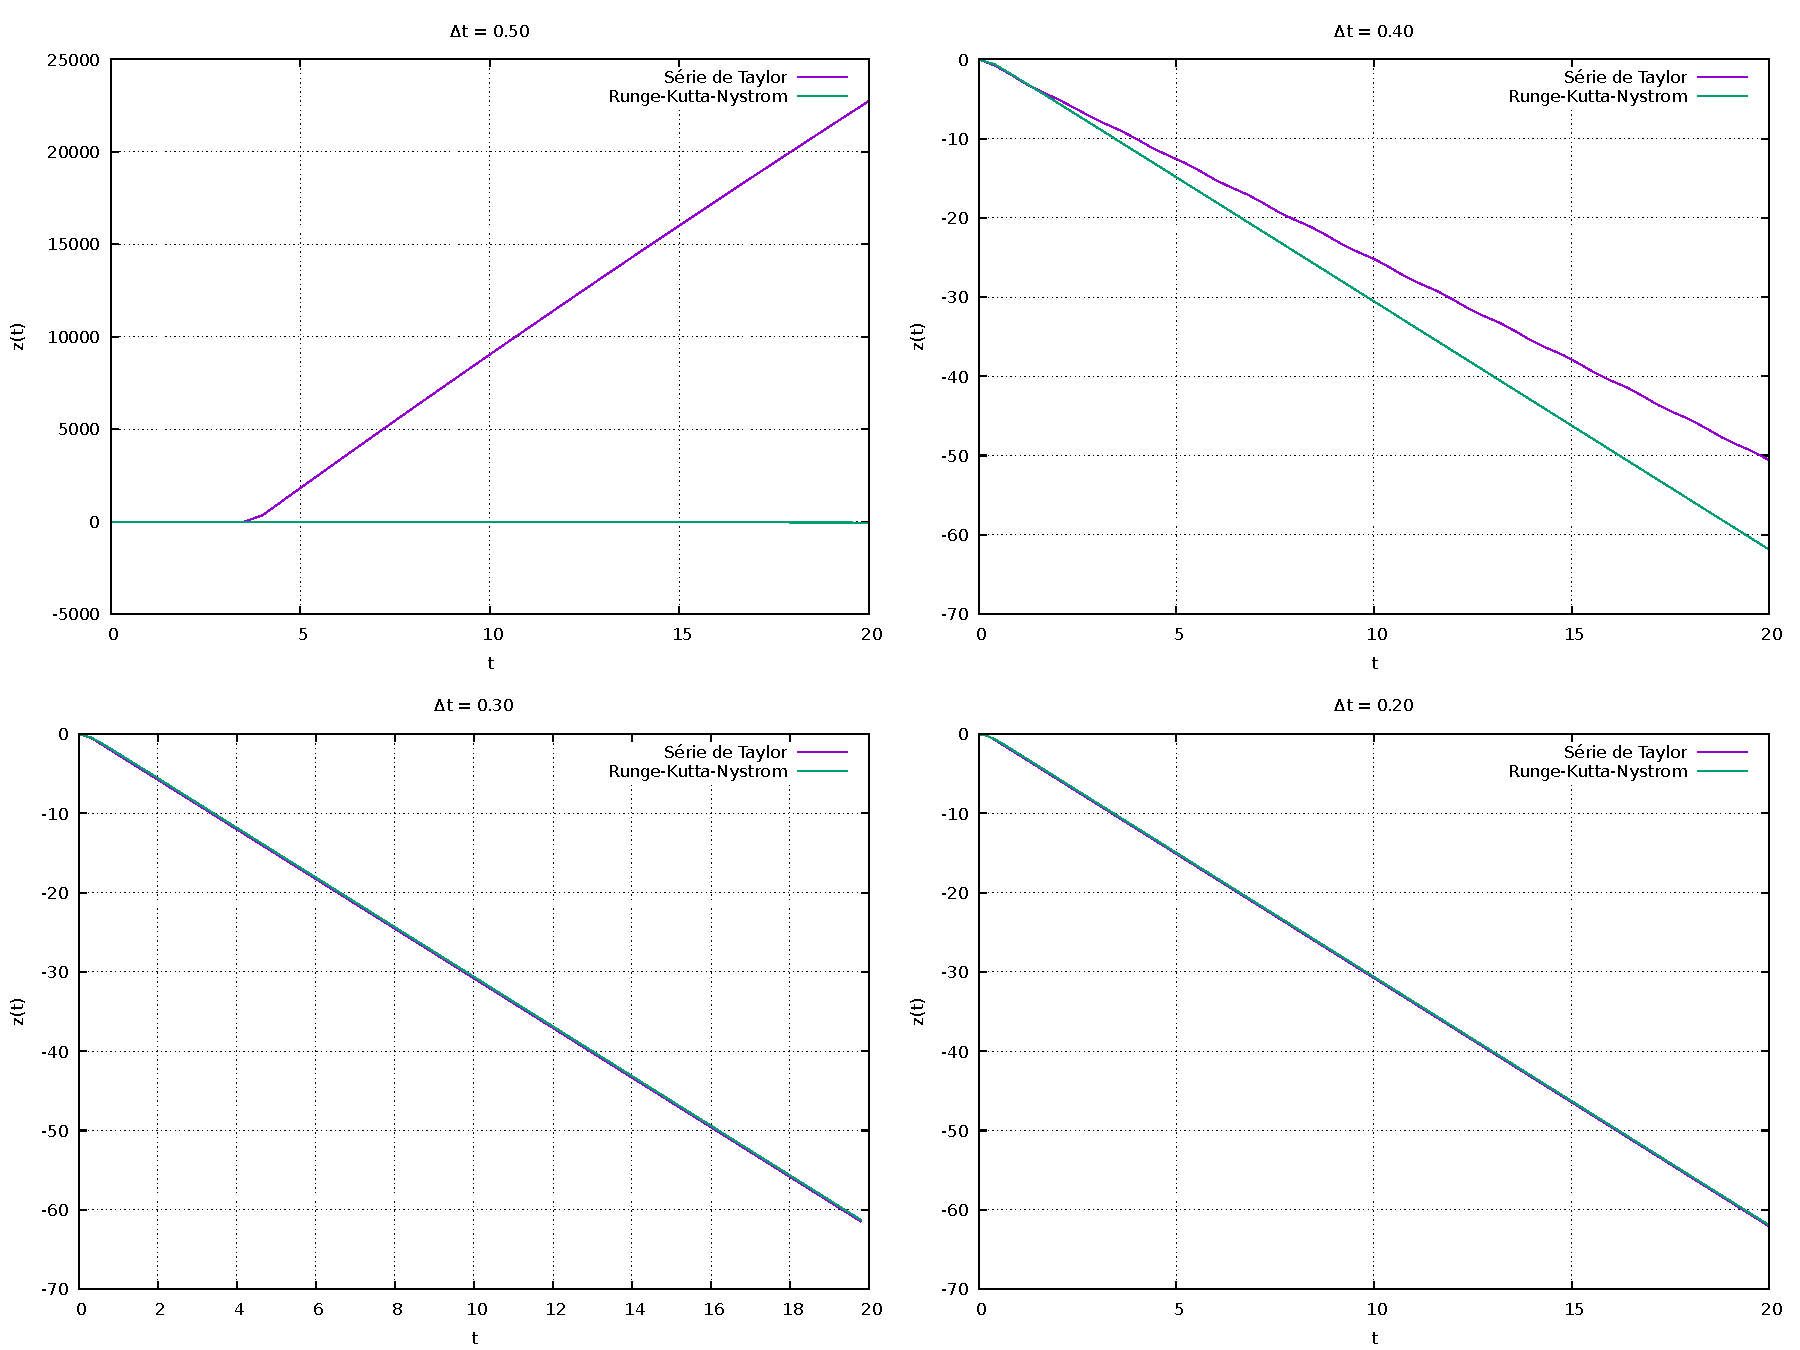
\includegraphics[width=\textwidth]{../src/plot/L6-Q3.pdf}
	\end{fig}

	Como dito em aula, esta equação modela o deslocamento horizontal de um objeto abandonado em repouso sobre a superfície da água. É interessante perceber como a aceleração $z''(t)$ aumenta em módulo no sentido para baixo conforme a gravidade $g$, enquanto o termo $k \cdot z'(t) \cdot |z'(t)|$ representa o empuxo exercido pelo fluido: Uma vez que a velocidade é negativa (movimenta o objeto para o fundo), o sinal que antecede o produto torna este positivo, a fim de compensar o efeito da gravidade. A constante $k$ se apresenta como o grau de viscosidade do meio.

	\quest[Extra: Queda livre na água.]
	
	Pensando na interpretação física do problema, achei que seria interessante visualizar uma situação onde o objeto é abandonado de um ponto acima do nível da água. Escolhendo arbitrariamente, supus $z(0) = 100$, enquanto mantive $z'(0) = 0$. Além disso, a equação diferencial ordinária de segunda ordem precisou ser reescrita em partes, para os diferentes meios:
	$$ z''(t) = \begin{cases}
		- g & \text{ se } z \ge 0\\
		- g - k \cdot z'(t) \cdot |z'(t)| & \text{ se } z < 0\\
	\end{cases}$$
	Isso, é claro, desprezando a resistência do ar. Os resultados foram os seguintes:
	\begin{fig}
		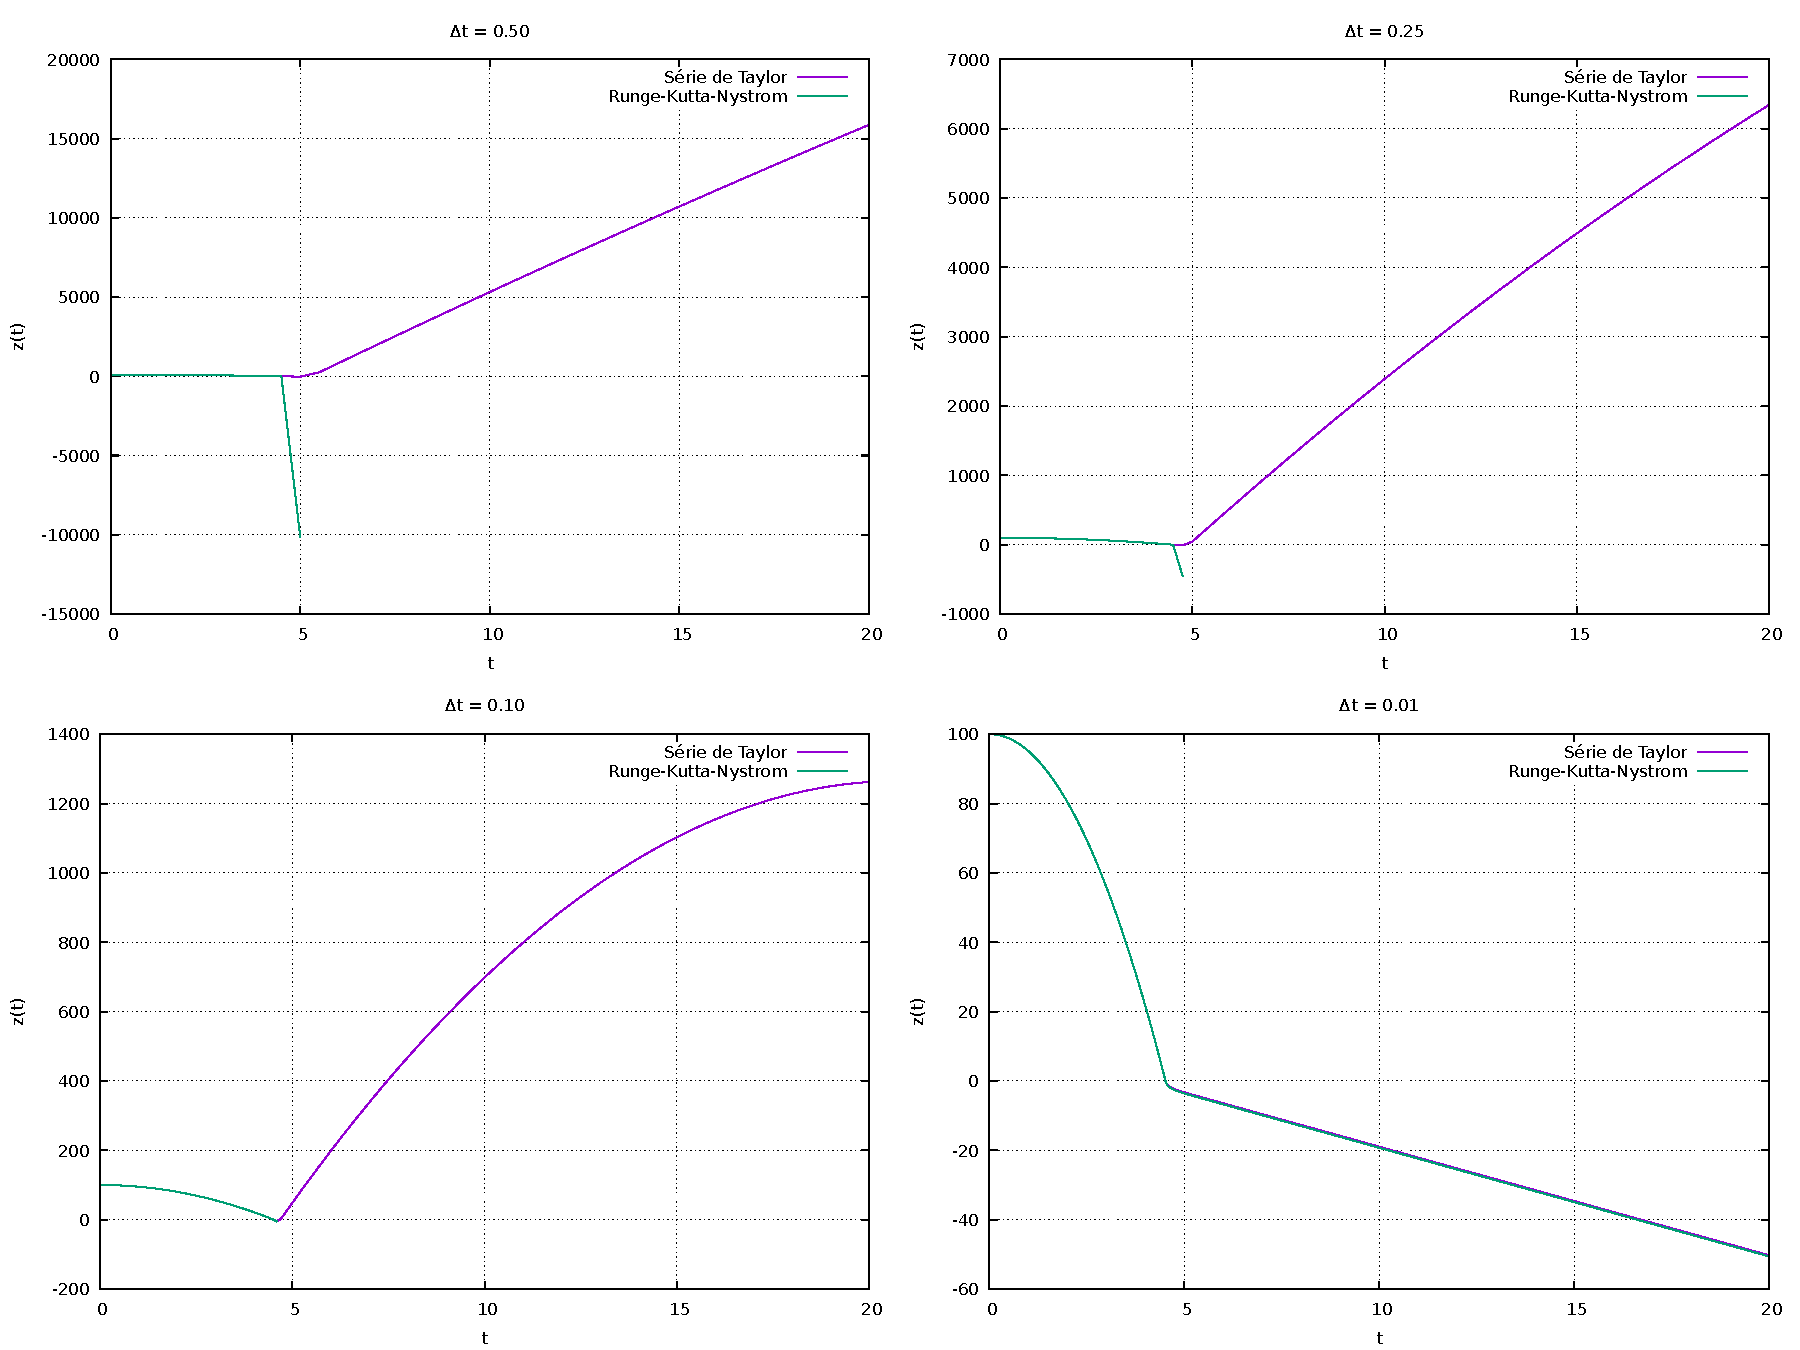
\includegraphics[width=\textwidth]{../src/plot/L6-QB.pdf}
	\end{fig}
	Como esperado, o gráfico da posição do objeto no tempo descreve uma parábola enquanto se encontra no ar e, após atravessar a linha d'água ($z = 0$), se comporta como no caso anterior. O que mais chamou minha atenção foi a divergência e instabilidade numérica para passos da ordem de $\Delta t = 10^{-1}$, faixa na qual os algoritmos se comportaram bem anteriormente.\par
	%%
	Achei interessante ver nestes gráficos o "impacto" do objeto sobre a água, causado pela descontinuidade imposta sobre a segunda derivada $z''(t)$.
	

	\pagebreak
	\appendixpage
	\appendix \section*{Código - Programa Principal}
	\lstinputlisting[style=fortranstyle, gobble=0]{../src/main5.f95}
	\appendix \section*{Código - Definição das Funções}
	\lstinputlisting[style=fortranstyle, gobble=0]{../src/funcmod.f95}
	\appendix \section*{Código - Métodos Numéricos}
	\lstinputlisting[style=fortranstyle, gobble=0]{../src/calclib.f95}
	\appendix \section*{Código - Métodos com Matrizes}
	\lstinputlisting[style=fortranstyle, gobble=0]{../src/matrixlib.f95}
	\appendix \section*{Código - Biblioteca Auxiliar}
	\lstinputlisting[style=fortranstyle, gobble=0]{../src/utillib.f95}
	\appendix \section*{Código - Biblioteca de Plotagem}
	\lstinputlisting[style=fortranstyle, gobble=0]{../src/plotlib.f95}
%	\begin{thebibliography}{10}
%		
%	\end{thebibliography}
\end{document}
